% !TEX ROOT=./main.tex



\section{Numerical Experiments}


% \begin{figure}
% \begin{tabular}{cc}
% 	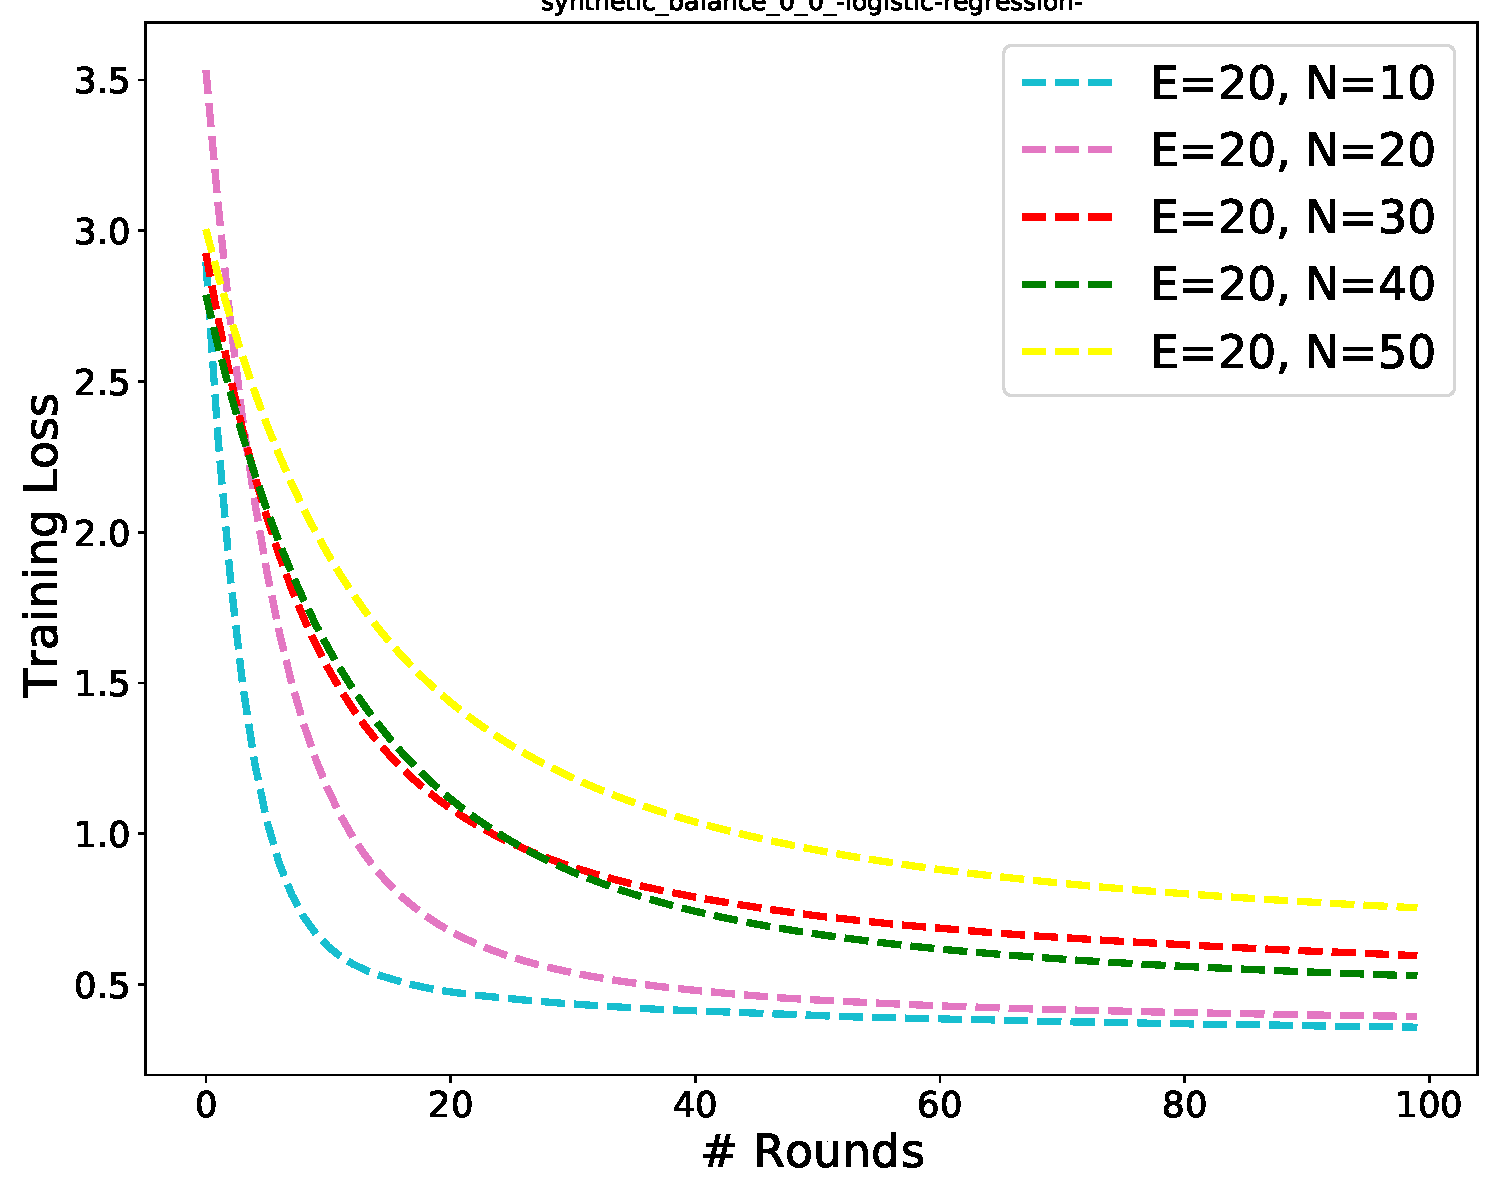
\includegraphics[width=0.5\textwidth]{fig/synthetic_balance_0_0_loss.pdf} & 
% 	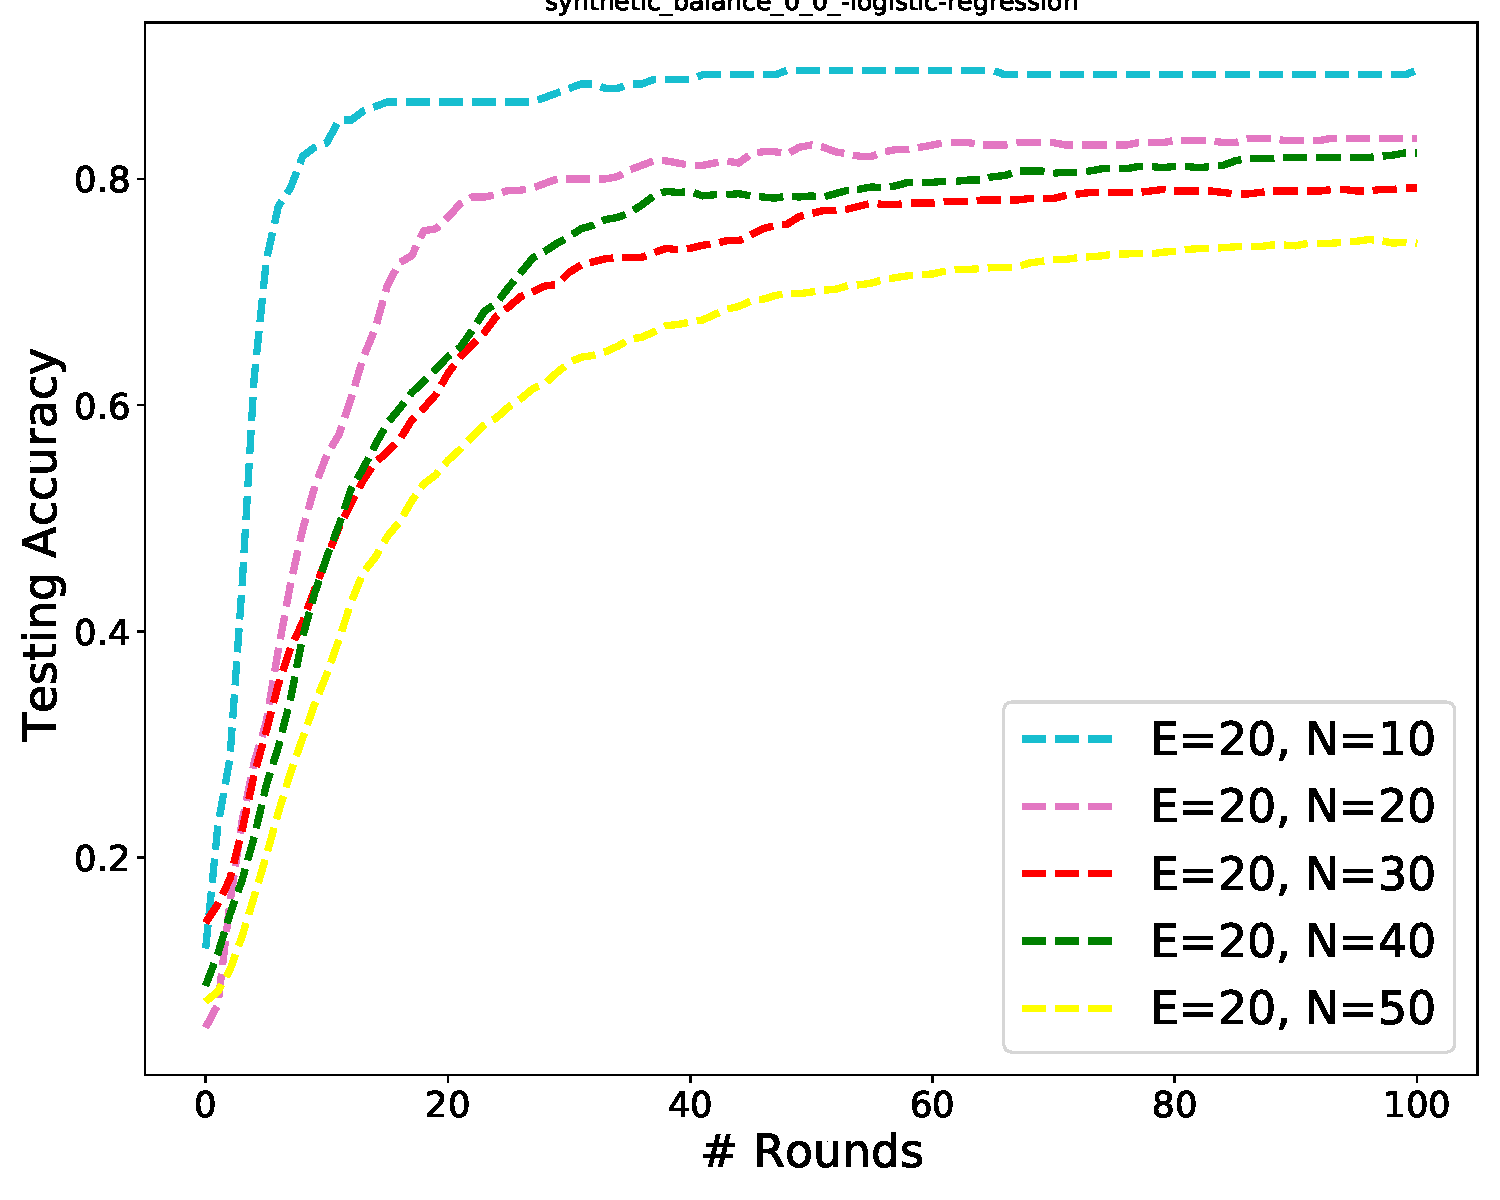
\includegraphics[width=0.5\textwidth]{fig/synthetic_balance_0_0_accuracy.pdf} \\
% 	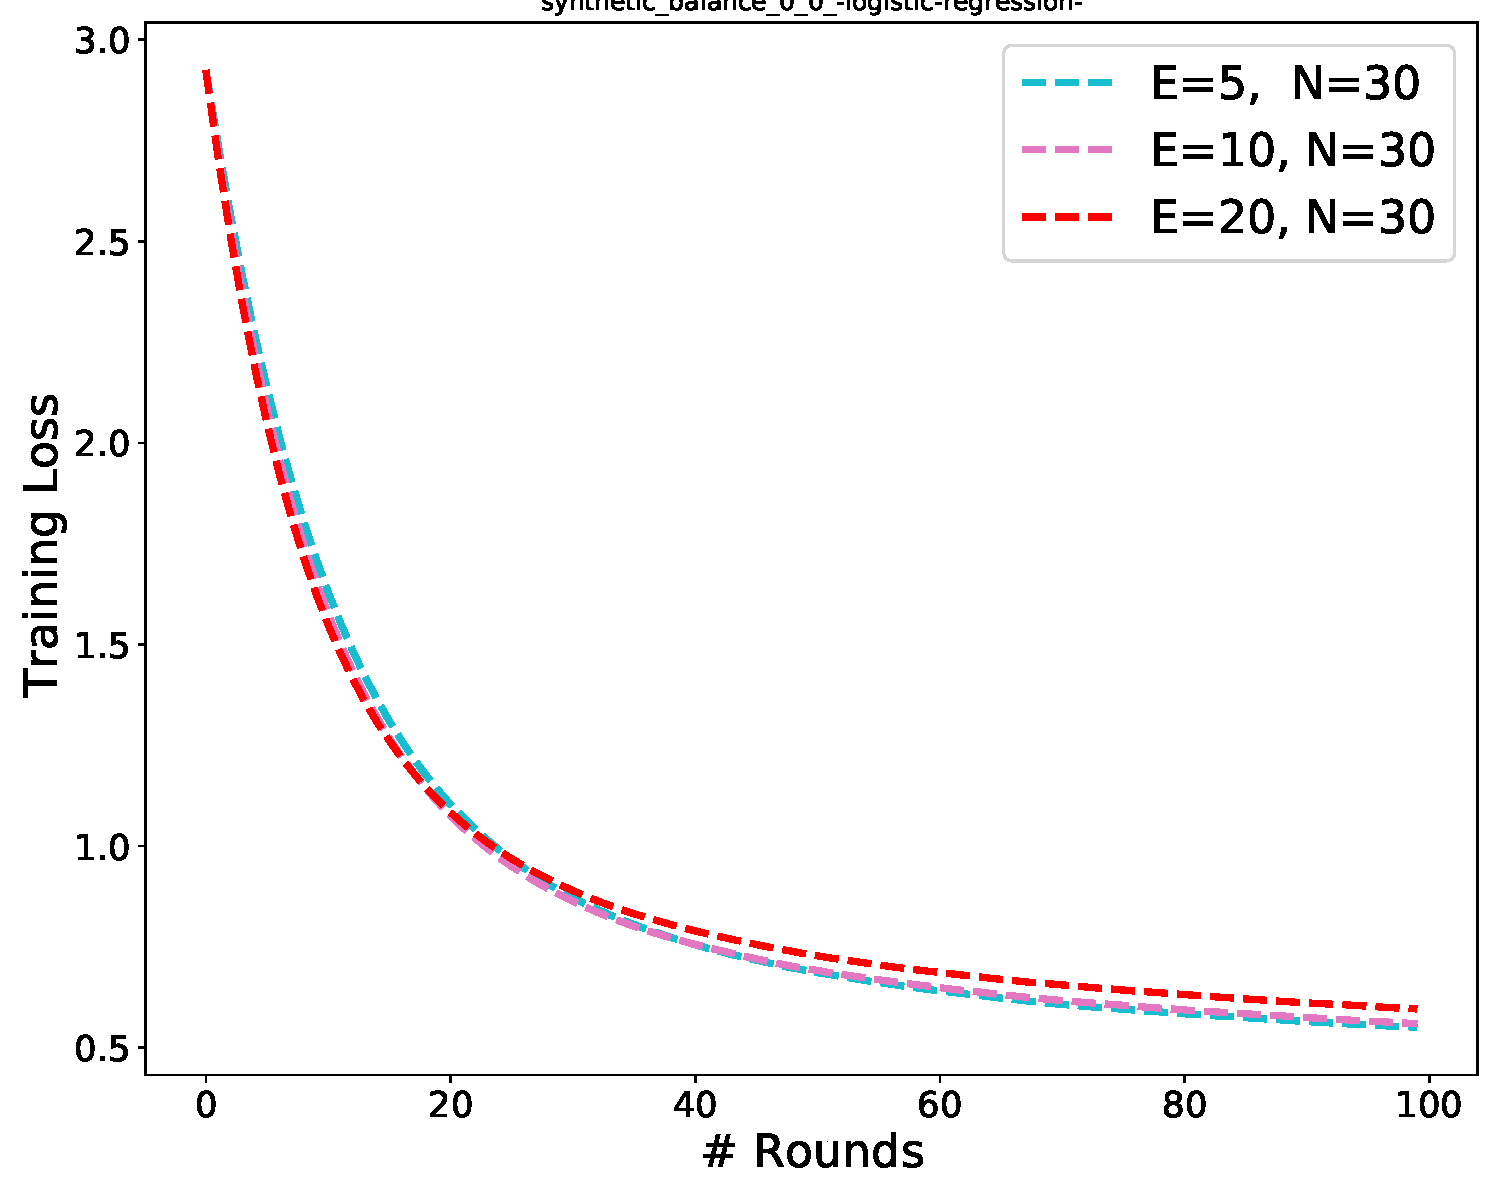
\includegraphics[width=0.5\textwidth]{fig/synthetic_balance_0_0_lossuser30TuneE.pdf} & 
% 	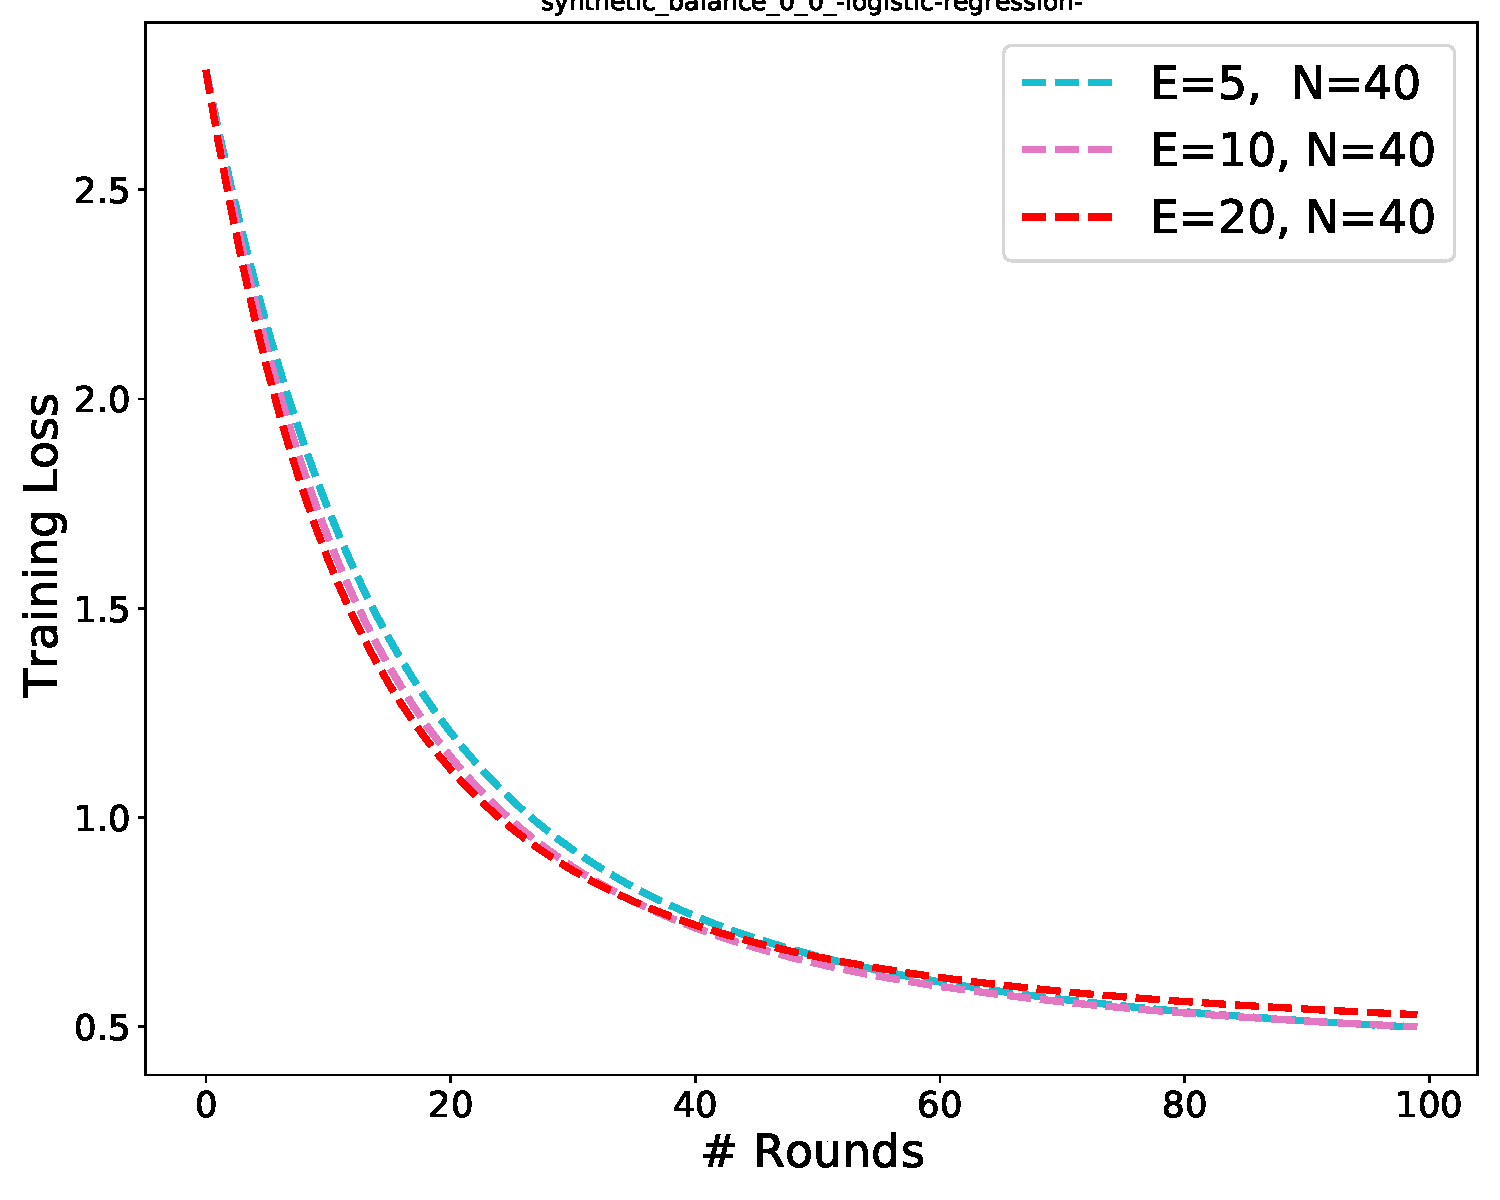
\includegraphics[width=0.5\textwidth]{fig/synthetic_balance_0_0_lossuser40TuneE.pdf} \\
% \end{tabular}
% \caption{Each user has 250 samples, non-iid setting, full device participation. Constant learning rate 0.01.}
% \end{figure}

We examine the practical speedup on a linear regression problem, 
$ F(\vw) = \sum_{k=1}^N p_kF_k(\vw)$, the objective function on each local device $k$ is given by, $F_k(\vw) = \frac{1}{N_k} \sum_{i=1}^{N_k} (\vw^T\vx_i^k + b  - y_i^k)^2$, where we generated i.i.d. data $\vx_i^k$ for all devices. At each communication round, all devices participated
in synchronization. 

\begin{figure}
\centering
\begin{tabular}{cc}
	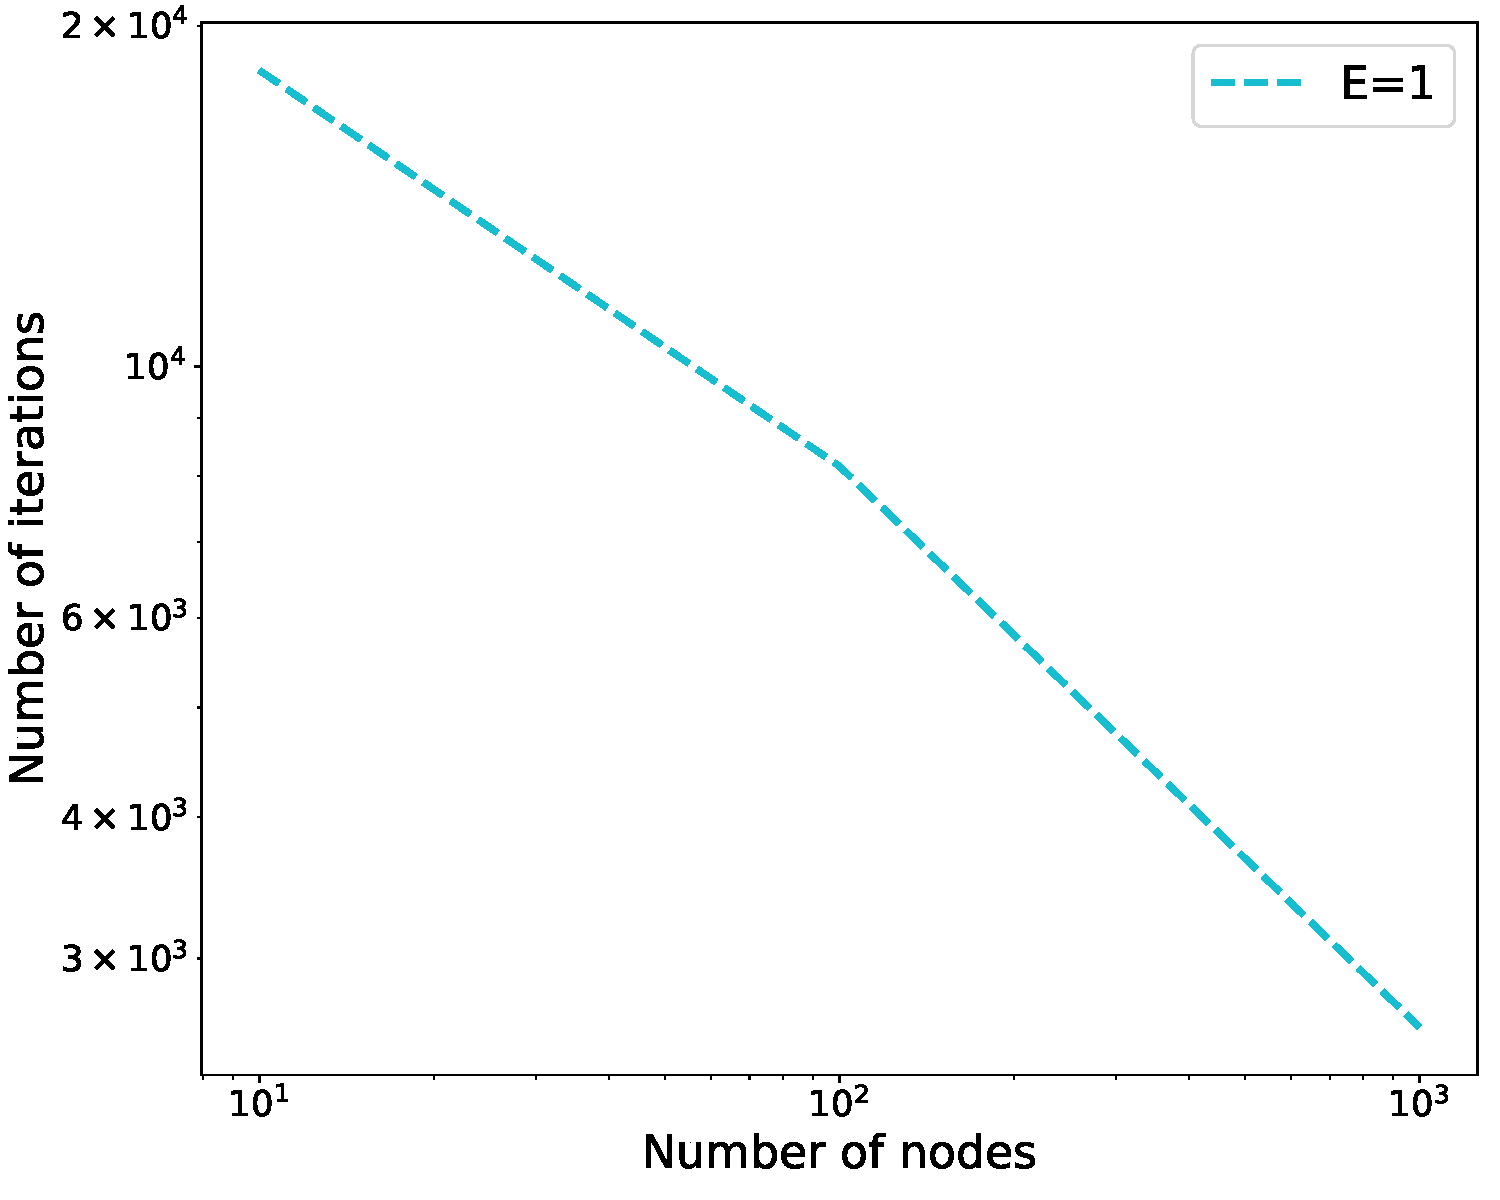
\includegraphics[width=0.5\textwidth]{fig/synthetic_linear_regression_1k_6k-epsilon01-logTrue.pdf} & 
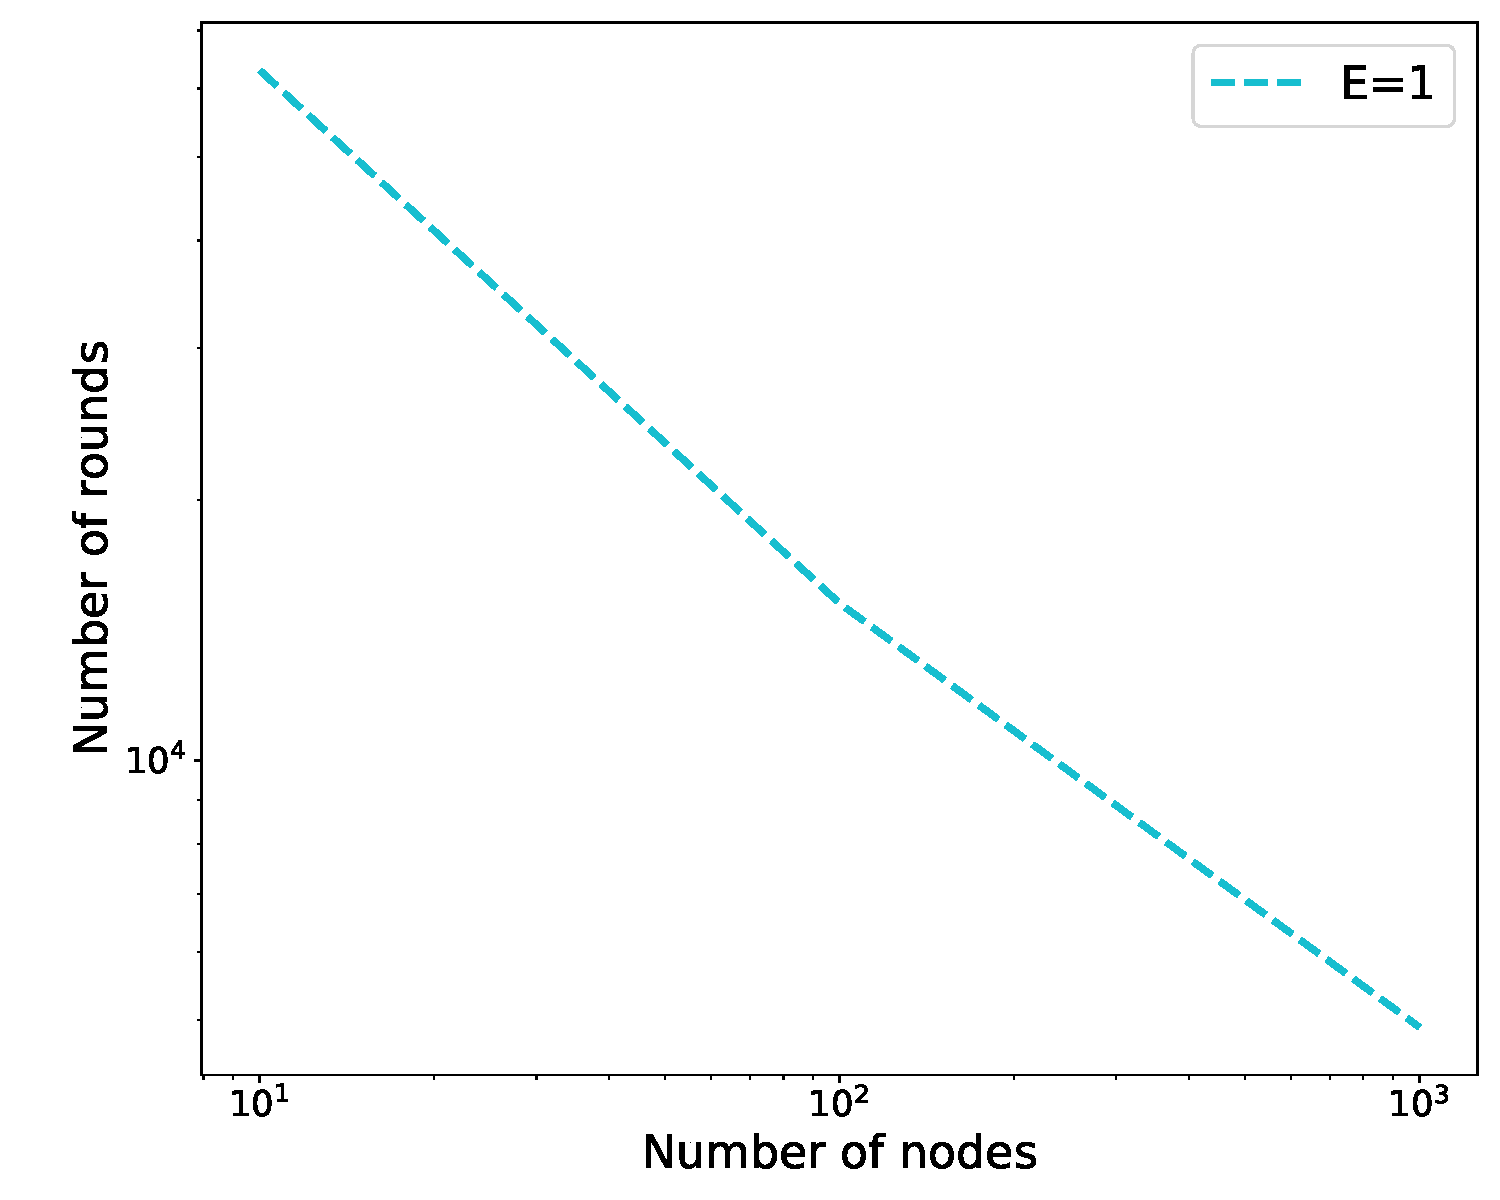
\includegraphics[width=0.5\textwidth]{fig/synthetic_linear_regression_1k_6k-epsilon001-logTrue-epoch-1.pdf} \\
(a) $\epsilon=0.01$  & (b) $\epsilon=0.001$
\end{tabular}
	\caption{The linear speed up w.r.t the number of nodes. The synthetic dataset has $6000$ samples, evenly distributed on $10, 100, 1000$ devices. The figure shows the number of iterations needed to converge to $\epsilon$. The learning rate is decayed as the $\eta_t = \frac{1}{c + t \times a}$, where we extensively search the best learning rate $c \in \{1, 10\}$ and $a \in \{1\mathrm{e}{-2}, 1\mathrm{e}{-3}, 1\mathrm{e}{-4}, 1\mathrm{e}{-5}, 1\mathrm{e}{-6}\}$ for each configuration.}
\end{figure}

